El programa desarrollado para el análisis de películas radiocrómicas proporciona varias funcionalidades para el usuario. En la figura \ref{fig:ventanaPrincipal} se muestra la ventana principal del programa.\\
\begin{figure}[H]
	\centering
	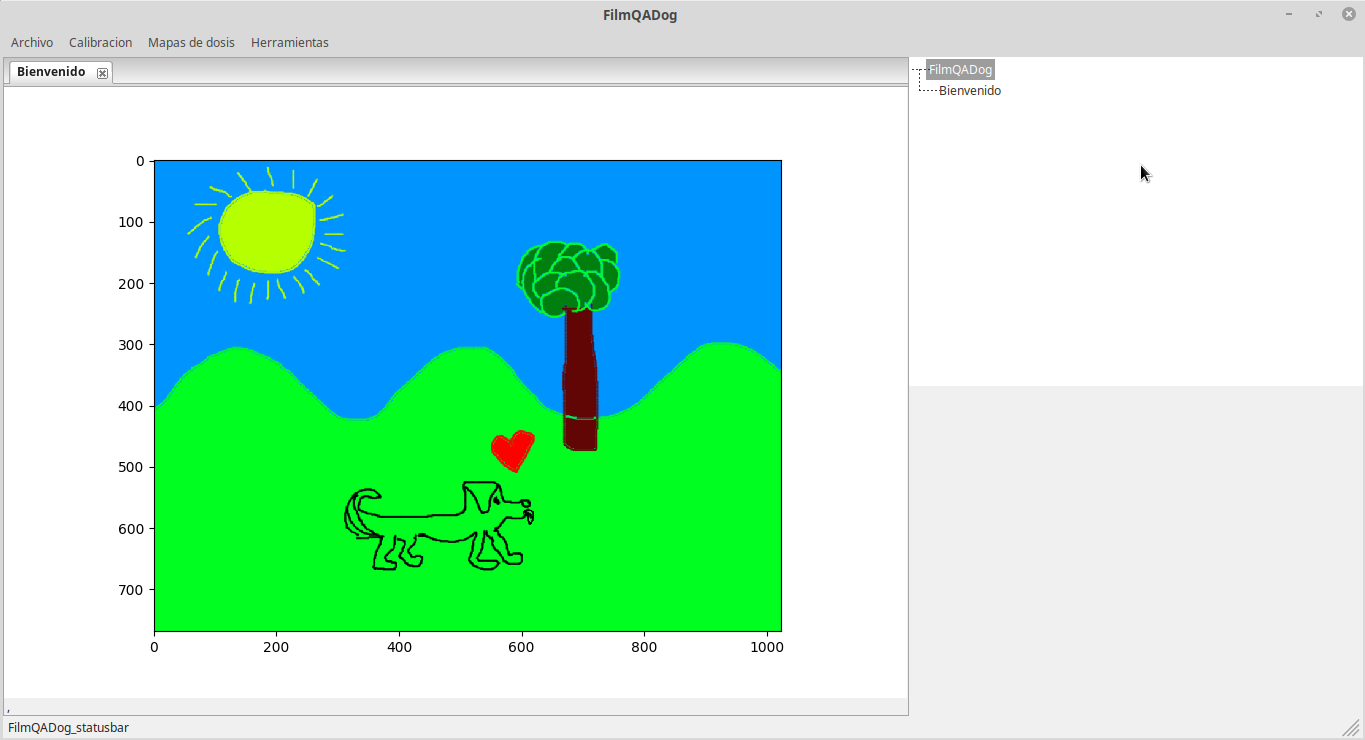
\includegraphics[width=0.7\linewidth]{images/imagenesDocumentacion/ventanaPrincipal.png}
	\caption{Ventana principal. }
	\label{fig:ventanaPrincipal}
\end{figure}

En el menú superior se encuentran categorizadas las diversas funcionalidades que se requieren para realizar un análisis con películas radiocrómicas. En la parte derecha se encuentra un árbol de archivos que permite navegar entre los archivos abiertos actualmente en el programa, además del espacio del panel de control, donde se van a ubicar los botones de control dependiendo de la función requerida.\\

El primer menú permite realizar la calibración bajo diferentes configuraciones, a partir de una serie de películas irradiadas con diferentes dosis escaneadas en un formato tiff. En la figura \ref{fig:menuCalibracion} se muestran las diferentes opciones de configuración a las cuales el usuario tiene acceso.\\
\begin{figure}[H]
	\centering
	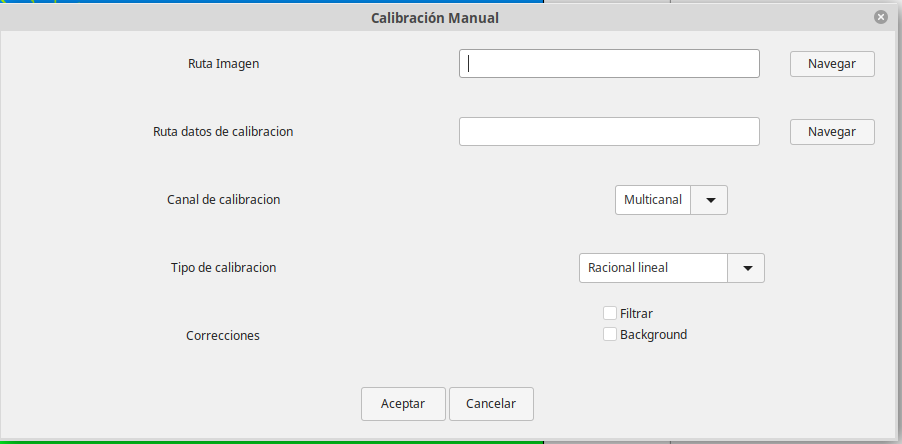
\includegraphics[width=0.7\linewidth]{images/imagenesDocumentacion/menuCalibracion.png}
	\caption{Menú de calibración. }
	\label{fig:menuCalibracion}
\end{figure}

Después de la elección de configuración, se procede a la ventana de selección de ROIs que se usarán en la calibración. Esta ventana se muestra en la imagen \ref{fig:menuEleccionDosis}.
\begin{figure}[H]
	\centering
	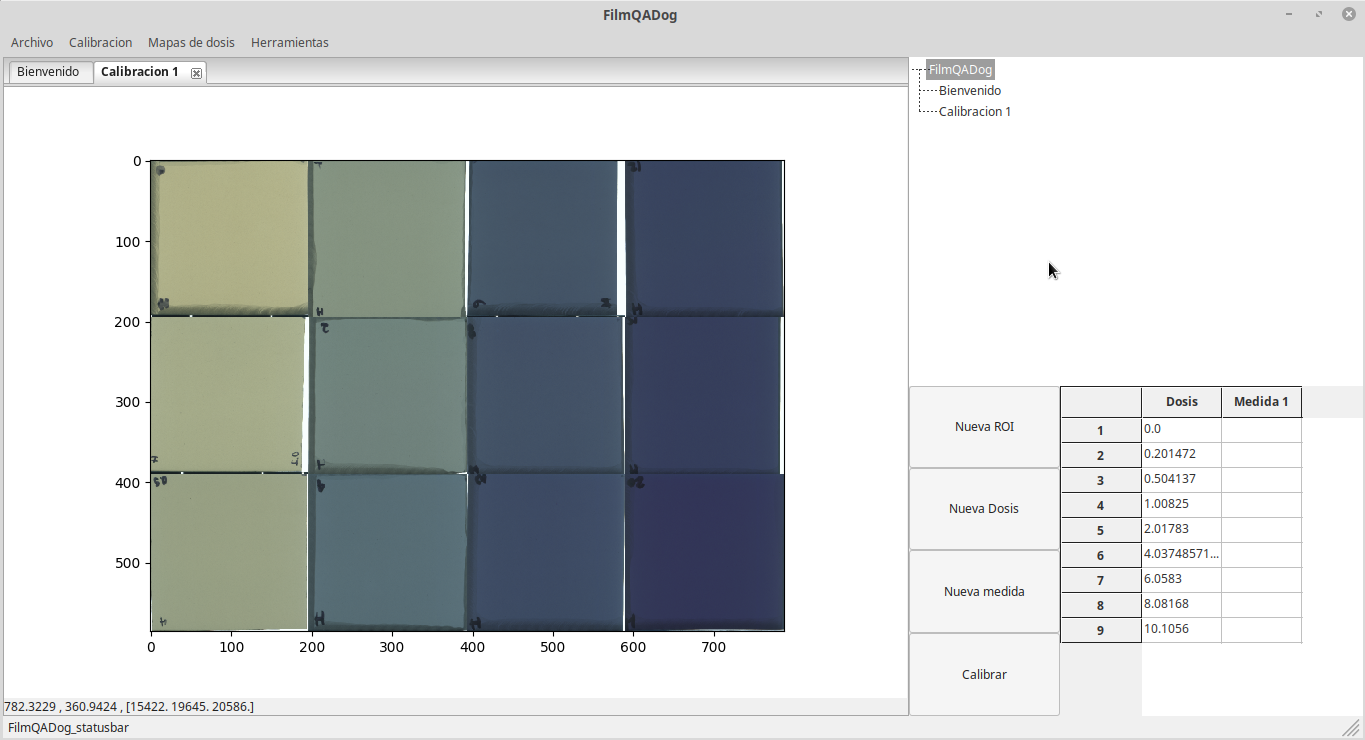
\includegraphics[width=0.7\linewidth]{images/imagenesDocumentacion/menuEleccionDosis.png}
	\caption{Ventana de selección de ROI. }
	\label{fig:menuEleccionDosis}
\end{figure}
Pulsando el botón de calibrar se creará un archivo de calibración(con extensión .calibr) que contiene la información del ajuste realizado con los datos que se consignan en la tabla mediante la interacción con la interfaz. Cada vez que se presione el botón de Nuevo ROI se promediara en la imagen las transmitancias del área elegida y se consignará este valor en la tabla.\\

En el menú de generación de mapas de dosis, al que se accede seleccionando el botón en la barra menú superior y que se muestra en la figura \ref{fig:menuMapaDosis} se elije un archivo de calibración y una imagen de una película escaneada en formato tiff. Además se eligen las opciones de filtros y correcciones por background.\\
\begin{figure}[H]
	\centering
	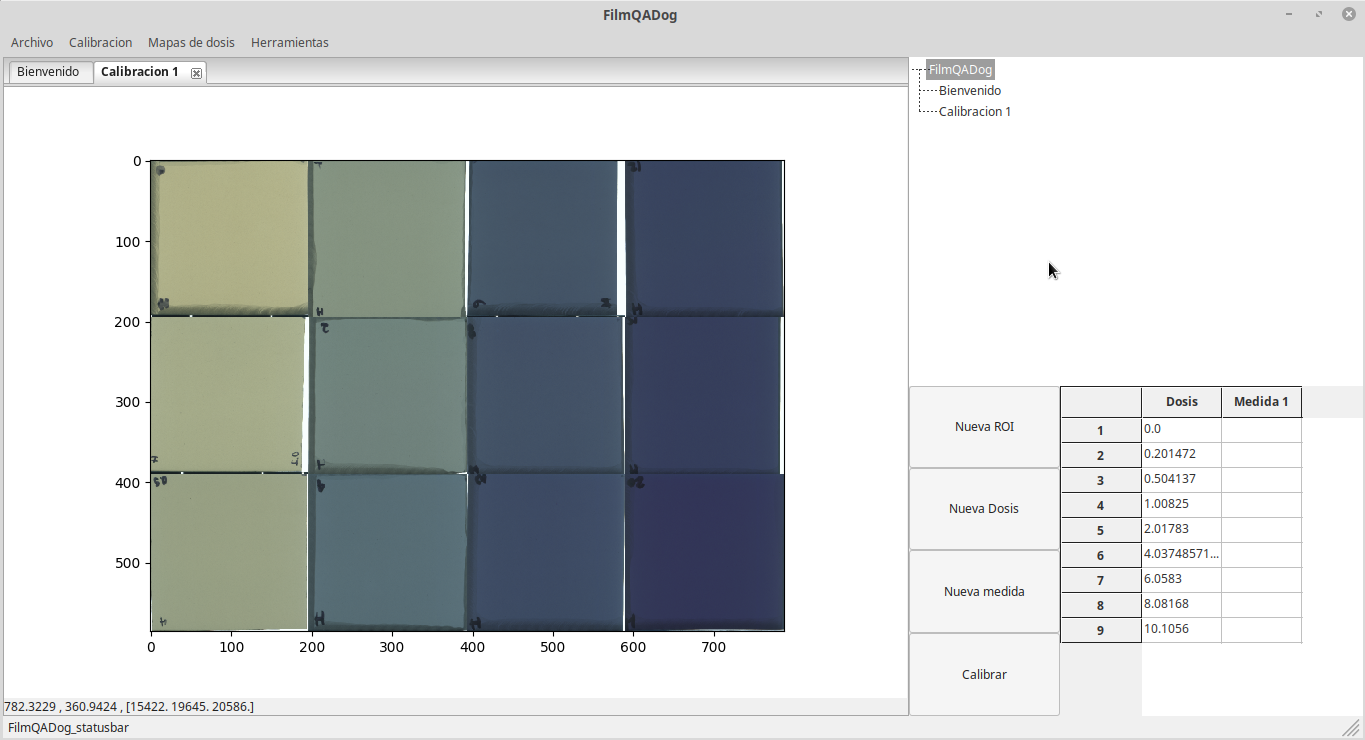
\includegraphics[width=0.7\linewidth]{images/imagenesDocumentacion/menuEleccionDosis.png}
	\caption{Menú para elección de características mapa de dosis. }
	\label{fig:menuMapaDosis}
\end{figure}

Después de seleccionados estos parámetros se abre una ventana donde se muestra la película seleccionada, teniendo la opción de seleccionar y remover puntos fiduciarios, así como elegir solo una sección de esta para analizar. Esta ventana se muestra en la figura \ref{fig:ventanaMapaDosis1}.\\
\begin{figure}[H]
	\centering
	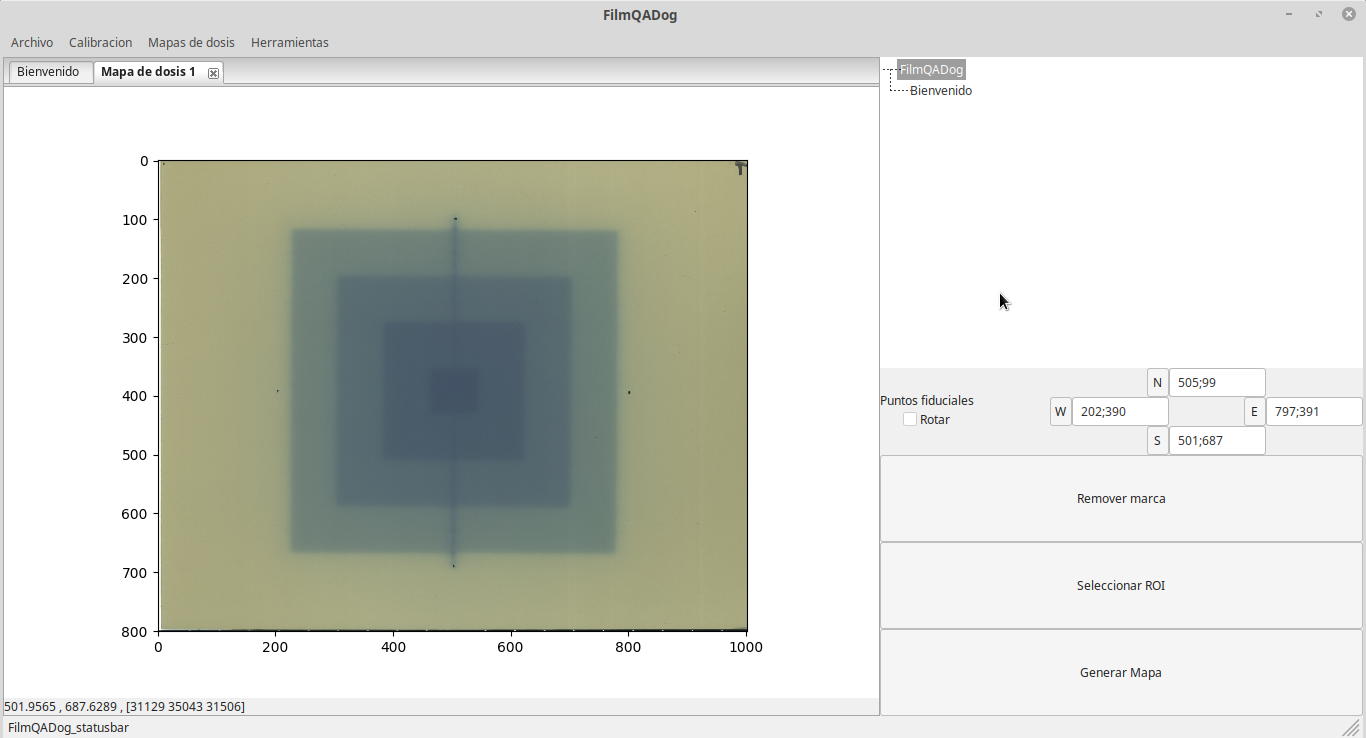
\includegraphics[width=0.7\linewidth]{images/imagenesDocumentacion/ventanaMapaDosis.png}
	\caption{Primera ventana para generación de mapas de dosis. }
	\label{fig:ventanaMapaDosis1}
\end{figure}

Una vez se presione el botón de generar mapa, se realizará la conversión del área de la imagen seleccionada al mapa de dosis mediante la información del archivo de calibración seleccionado. Este mapa creado se muestra en otra ventana, que se ilustra en la figura \ref{fig:ventanaMapaDosis2}, y provee diversas opciones para el análisis del mismo. Así, se puede realizar un análisis interactivo de perfiles de dosis, histogramas de dosis y curvas de isodosis. También, se puede cambiar el punto de normalización de los mapas eligiendo entre tres opciones posibles. Finalmente, el botón guardar mapa empaquetará este mapa en formato DICOM y lo guardará en el disco.\\

\begin{figure}[H]
	\centering
	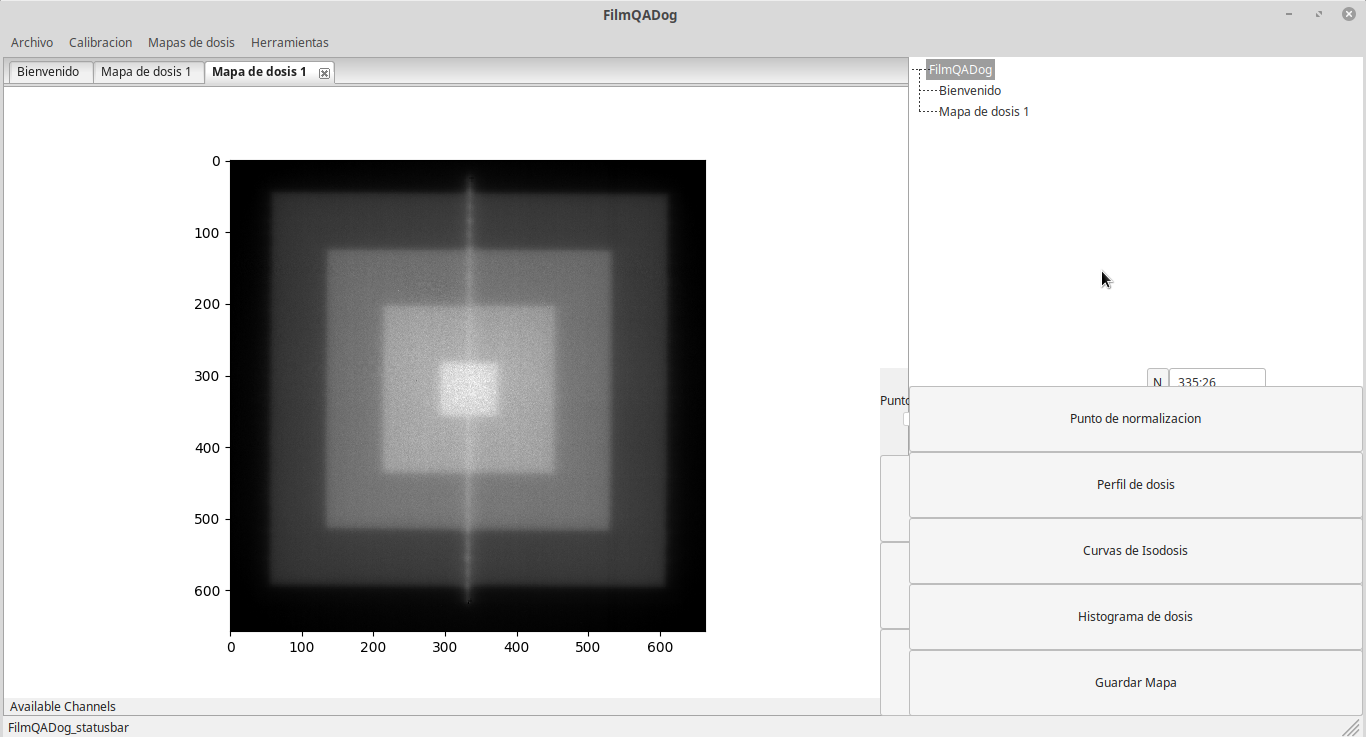
\includegraphics[width=0.7\linewidth]{images/imagenesDocumentacion/ventanaMapaDosis2.png}
	\caption{Segunda ventana para generación de mapas de dosis. }
	\label{fig:ventanaMapaDosis2}
\end{figure}

Por último, el menú de comparación a plan, al que se accede por la barra menú en la parte superior, muestra las opciones que se pueden modificar para realizar el análisis $\Gamma$. Este menú se muestra en la figura \ref{fig:menuComparacion}.

\begin{figure}[H]
	\centering
	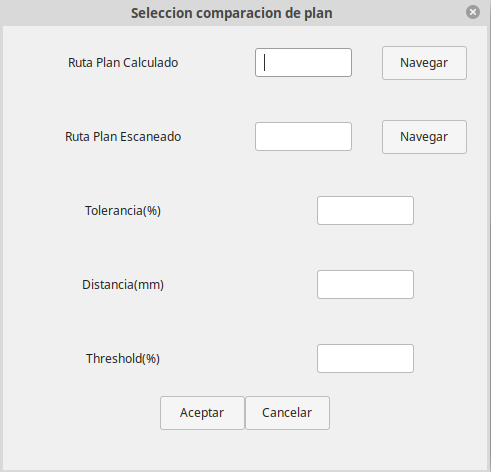
\includegraphics[width=0.7\linewidth]{images/imagenesDocumentacion/menuComparacionAplan.png}
	\caption{Menú para elegir las propiedades de comparación. }
	\label{fig:menuComparacion}
\end{figure}

Lo cual abre una ventana donde se superponen los planes calculados y escaneados, así como las diversas opciones de comparación, incluyendo el análisis $\Gamma$ que se puede realizar. Esta última ventana se muestra en la figura \ref{fig:ventanaComparacion}

\begin{figure}[H]
	\centering
	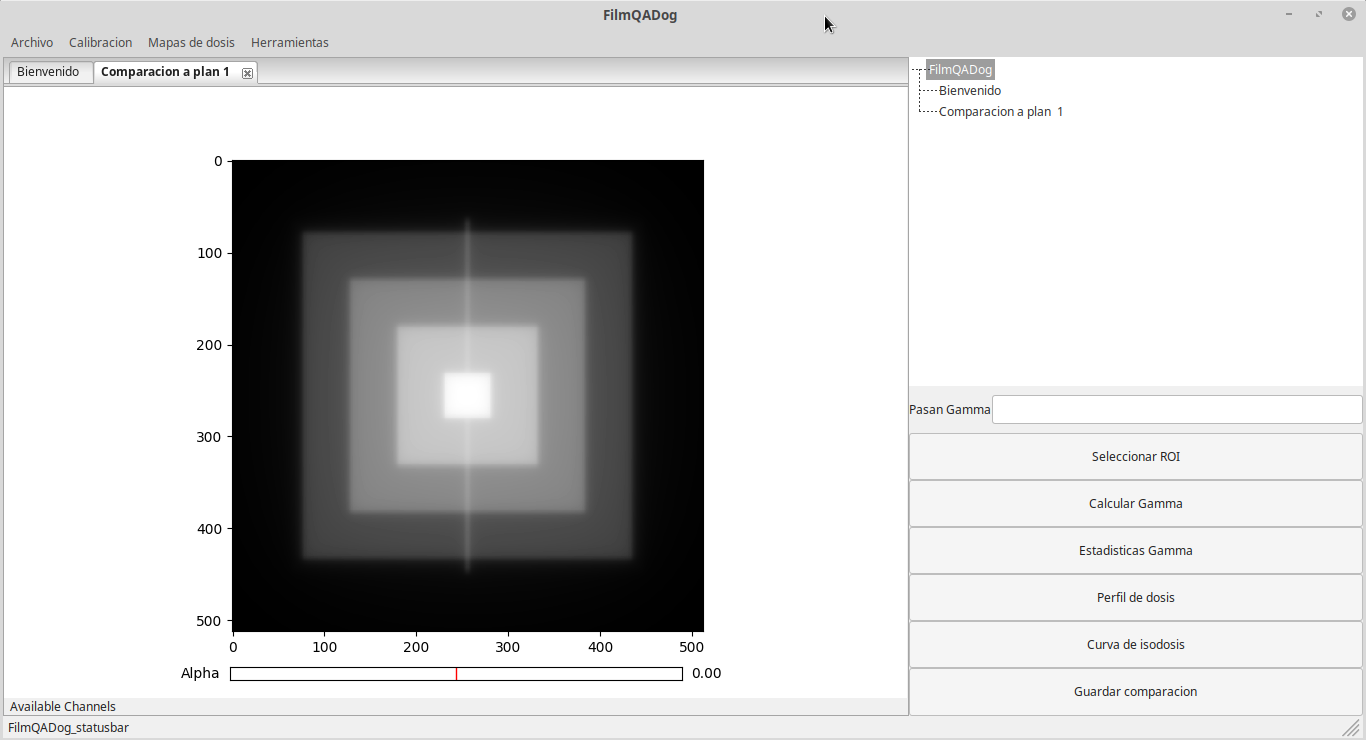
\includegraphics[width=0.7\linewidth]{images/imagenesDocumentacion/ventanaComparacioAPlan.png}
	\caption{Ventana con opciones de comparación. }
	\label{fig:ventanaComparacion}
\end{figure}

